\chapter{Adding Entries}
So, there are a number of ways to enter information into the database, below we will discuss each one in turn.

\section{Albums}
\label{sect:albums}
We add data by adding albums.  Select the 
\textit{\textbf{Add Album}}
button as shown in Figure 
\ref{fig:Add album}.
\begin{figure}[!ht]
 \centering
 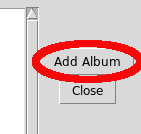
\includegraphics[scale=1]{albumButton2.png} 
 \caption{Add album}
 \label{fig:Add album}
\end{figure}

You should see the 
\textit{\textbf{New Album}}
screen (Figure 
\ref{fig:New album}).
\begin{figure}[!ht]
 \centering
 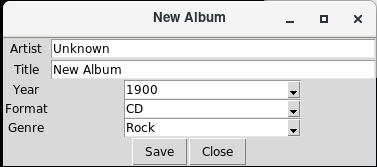
\includegraphics[width=\textwidth]{addAlbum.png}
 \caption{New album}
 \label{fig:New album}
\end{figure} 
This is the key to entering all the data into the database.
\newpage

\subsection{The first entry}
So, let's get on and enter that first album into our new database.  You will have noticed, from Figure
\ref{fig:New album},
that some details have been pre-populated.  When a new database is created the 
\textit{\textbf{Format}}
table is populated with an entry 
\textit{\textbf{CD}}, 
and the
\textit{\textbf{Genre}} 
table is populated with an entry 
\textit{\textbf{Rock}} 
\footnote{See Part II, Tables for  full details of the Database structure.},
as a convenience to get things started.  The 
\textit{\textbf{Label}} and 
\textit{\textbf{Original Label}}
drop downs are populated with
``\textit{\textbf{Enter/Choose a Record label}}''
\footnote{This was originally populated with \textit{\textbf{``Unknown''}}, but it turns out that \textit{\textbf{``Unknown Records''}} actually did exist.}
.  The 
\textit{\textbf{This Release}} and
\textit{\textbf{Original Release}}
drop downs are populated with every year from 1900 to the current year (see Figure 
\ref{fig:Year selection}).
\begin{figure}[!ht]
 \centering
 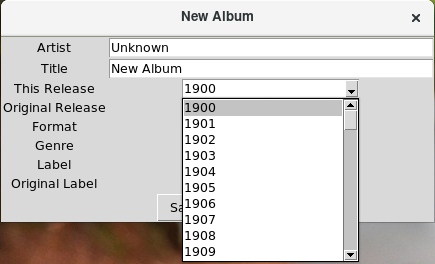
\includegraphics[width=\textwidth]{yearDropdown.png}
 \caption{Year selection}
 \label{fig:Year selection}
\end{figure}

\newpage 
For now, just to show off a few points, select
\textbf{\textit{Save}}.
Now our main screen should look like Figure
\ref{fig:First album entered},
\begin{figure}[!ht]
 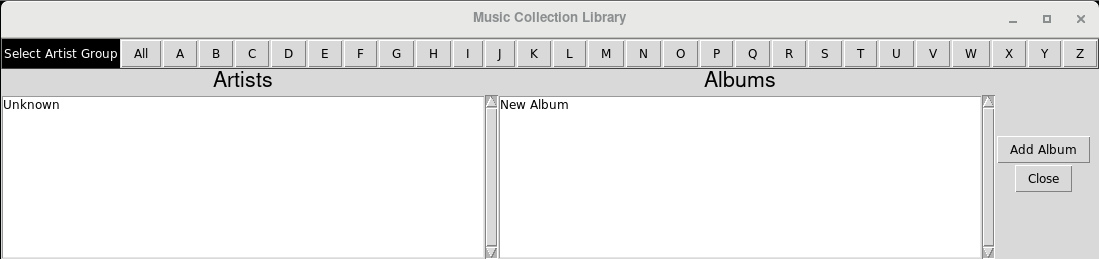
\includegraphics[width=\textwidth]{popFirstAlbum.png} 
 \caption{First album entered}
 \label{fig:First album entered}
\end{figure}
but really that's not much use to us, unless of course you have an album from 1900, on CD, in the rock genre, by a group called ``Unknown'', entitled ``New Album''.  So let's change those details to something sensible. Click on the album name and you should see the
\textit{\textbf{New Album}}
screen (Figure 
\ref{fig:New album})
again.  Complete the details as shown in Figure
\ref{fig:Sgt. Pepper's Lonely Hearts Club Band}
\begin{figure}[!ht]
 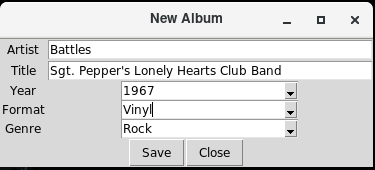
\includegraphics[width=\textwidth]{battlespepper.png}
 \caption{Sgt. Pepper's Lonely Hearts Club Band}
 \label{fig:Sgt. Pepper's Lonely Hearts Club Band}
\end{figure}
and click 
\textbf{\textit{Save}}.
You can enter
\textbf{\textit{Vinyl}}
by just clicking in the
\textbf{\textit{Format}}
text box and overwriting the
\textbf{\textit{CD}}
text, this will add
\textbf{\textit{Vinyl}}
to the drop down 
\textbf{\textit{Format}}
menu for future use.

Looking at the main screen it seems we messed up the Artist name (unless the Beatles changed their name in some strange time jump!), this is easily fixed: double click on the artist name and you will see the screen in Figure
\ref{fig:Edit artist}.
\begin{figure}[!ht]
 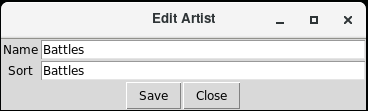
\includegraphics[scale=1]{editartist.png}
 \caption{Edit artist}
 \label{fig:Edit artist}
\end{figure} 
\newpage
Change the entries to ``Beatles'', or ``The Beatles'' if you prefer, see Figure
\ref{fig:Corrected artist}
\begin{figure}[!ht]
 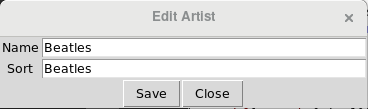
\includegraphics[scale=1]{editArtist2.png}
 \caption{Amend artist details}
 \label{fig:Corrected artist}
\end{figure} 
and click 
\textbf{\textit{Save}}.
\\You should now see something that looks like Figure
\ref{fig:Updated start screen}.
\begin{figure}[!ht]
 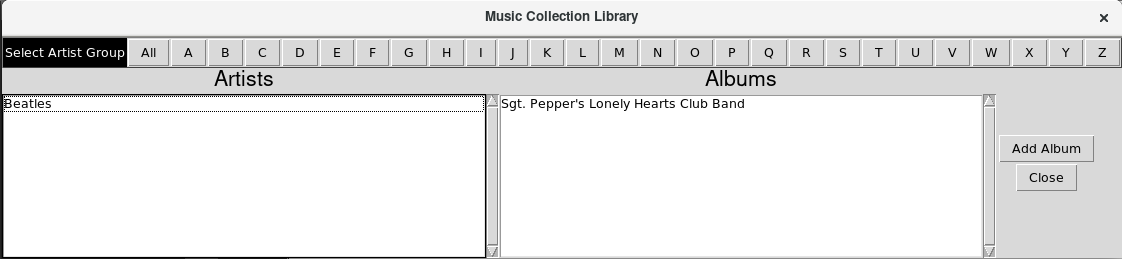
\includegraphics[width=\textwidth]{updatedMainScreen.png}
 \caption{The updated start screen}
 \label{fig:Updated start screen}
\end{figure} 

You might have noticed that we left the two
\textit{\textbf{Label}}
entries unchanged, let's fix that now so that our information is complete.  Click on the album name and you should see the
\textit{\textbf{New Album}}
screen (Figure 
\ref{fig:New album})
again.  Complete the details as shown in Figure
\ref{fig:Add the record label}
\begin{figure}[!ht]
 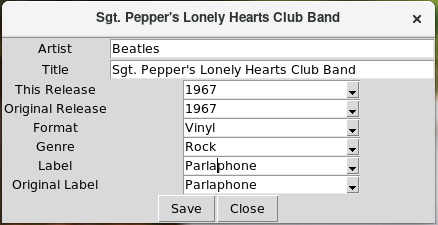
\includegraphics[width=\textwidth]{pepperlabel.png}
 \caption{Add the record label}
 \label{fig:Add the record label}
\end{figure}
and click 
\textbf{\textit{Save}}.

\newpage
Select the 
\textit{\textbf{Add Album}}
button, click on the down arrow to the left of the
\textit{\textbf{Label}}
entry box and you should see something like Figure
\ref{fig:Label selection}
\begin{figure}[!ht]
 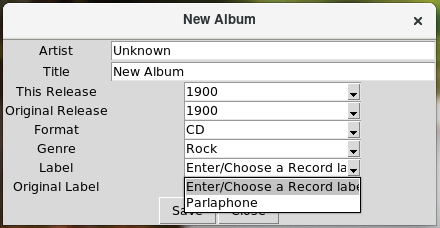
\includegraphics[width=\textwidth]{labelDropdown.png}
 \caption{Label selection}
 \label{fig:Label selection}
\end{figure} 
, every new record label you enter will be added to this list for selection on further additions to the library.  The
\textbf{\textit{Format}} and
\textbf{\textit{Genre}}
lists work in the same way.

\subsection{A word about release dates}
The two entries
\textbf{\textit{This Release}} and
\textbf{\textit{Original Release}}
are provided for quite specific reasons, and
\textbf{\textit{Original Release}}
plays an important role in the display of albums on the front page, indeed in the display of albums within an artists catalogue.
\textbf{\textit{This Release}}
is intended to be the release date of the specific medium referred to in this entry, whereas
\textbf{\textit{Original Release}}
should be the date that the recorded work was first released, as shown in Figure
\ref{fig:releaseDates}.
\begin{figure}[!ht]
 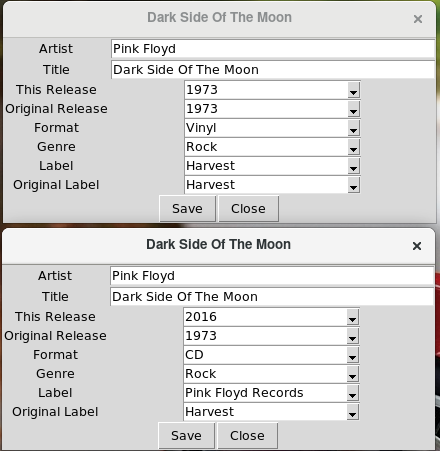
\includegraphics[width=\textwidth]{releaseDates.png}
 \caption{An example of release date usage}
 \label{fig:releaseDates}
\end{figure} 

Albums are listed in
\textbf{\textit{Original Release}}
date order.

\newpage
\section{Artists}
\label{sect:artists}
Artists are added to the database by entering album details, if the artist is not already in the database then they will be added.  You should maintain the sort field of the artists entry by double clicking the artist name from the front screen; this field is used to display the artists in alphabetical order. Figure
\ref{fig:exampleOfArtistSort} demonstrates.
\begin{figure}[!ht]
 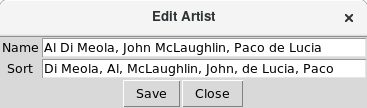
\includegraphics[width=\textwidth]{exampleOfArtistSort.png}
 \caption{An example of the artist sort field}
 \label{fig:exampleOfArtistSort}
\end{figure} 

\section{CSV}
\label{sect:csv}
The final method of inputting data to the database is by bulk loading details from a
\textbf{C}omma 
\textbf{S}eparated
\textbf{V}alues
file (
\textbf{CSV}).
As the name implies the data is held in a plain text file with a comma
(\textbf{,})
between each item.
\textbf{Mucollib}
will import data records from a CSV file named ``Music.csv''
\footnote{``Music.csv'' is currently hard-coded in the program.}
.  This option is offered when the program is first run and it does not find its database
(\textbf{music.db}), 
as shown in Figure 
\ref{fig:No database found}.
\begin{figure}[!ht]
  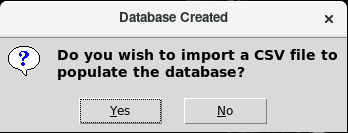
\includegraphics[width=\textwidth]{firstRun.png}
  \caption{No database found on first run}
  \label{fig:No database found}
\end{figure}
\newpage
The \textbf{CSV} file is subject to certain rules:
\begin{itemize}
\item each line represents one record to be entered into the database
\item each comma-separated value is an item of data
\item items containing commas (,) must be surrounded by quotation marks (``''), for example:
\begin{itemize}
\item \textit{John Martyn,``Martyn, John'',...}
\end{itemize}
\item the first line of the file is special, and is actually ignored by the data import, as it contains a description of the data item in that column, so:
\begin{itemize}
\item \textit{Artist,Sort,Album,Format,Genre,Year,Released,Label,OLabel}
\footnote{These headings are those used by the author, feel free to use any heading that is meaningful to you, the line is discarded anyway.}
\end{itemize}
\end{itemize}

So a typical csv file might contain data like the following:
\begingroup
\fontsize{8pt}{8pt}
\begin{itemize}
\item \textit{ArtistName,ArtistSort,AlbumName,Format,Genre,Year,Oyear,Label,Olabel}
\item \textit{AC/DC,AC/DC,For Those About To Rock,CD,Rock,1994,1981,Atlantic,Atlantic}
\item \textit{Tori Amos,"Amos, Tori",Under The Pink,CD,Rock,1994,1994,Atlantic,Atlantic}
\item \textit{Joan Armatrading,"Armatrading, Joan",Joan Armatrading,Vinyl,Rock,1976,1976,A\&M,A\&M}
\item \textit{Kevin Ayers,"Ayers, Kevin","June 1, 1974",Vinyl,Rock,1974,1974,Island,Island}
\end{itemize}
\endgroup
